%\section{Model formulation}

In this section, I outline the primary contribution of this work and develop a weighted likelihood approach for semi-supervised learning in HMMs. %The primary issue is that the likelihood in Equation (\ref{eqn:HMM_like_marginal}) is a product of matrices, so raising individual terms to a particular power is not straightforward. In this section, I address this issue in three steps. First, I write down the likelihood of a partially observed HMM. Next, I reparameterize and rescale the weighted likelihood from Equation (\ref{eqn:like_partial}). Finally, I use that re-parameterized and re-scaled likelihood to introduce a novel 
I begin by writing down the likelihood of a partially observed HMM. I use the same notation from Section 2.2, namely random labels $\bfZ = \{Z_t\}_{t \in \calT}$, where $Z_t$ is generated from hidden state $X_t$ and, conditioned on $\bfX$, $\bfY$, and $\bfZ \setminus \{Z_t\}$, depends only on $X_t$. As before, a fixed realization of $\bfZ$ is denoted as $\bfz = \{z_t\}_{t \in \calT}$, and I abuse notation by setting $z_t = \emptyset$ for all unlabelled observations (i.e., $t \notin \calT$) and $g^{(i)}(\emptyset ; \beta^{(i)}) = 1$. The HMM likelihood for observations $\bfy$ and labels $\bfz$ is thus
%
\begin{equation}
    p(\bfy,\bfz ~;~ \bfdelta, \bfGamma, \bftheta,\bfbeta) = \bfdelta P(y_1,z_1;\bftheta,\bfbeta) \prod_{t=2}^T \bfGamma P(y_t,z_t;\bftheta,\bfbeta) \mathbf{1}^\top_N, \label{eqn:PHMM_like}
\end{equation}
%
where $P_t(y_t,z_t;\bftheta,\bfbeta)$ is an $N \times N$ diagonal matrix with entry $(i,i)$ equal to $f^{(i)}(y_t; \theta^{(i)}) g^{(i)}(z_t; \beta^{(i)})$. I refer to this model as a \textit{partially hidden Markov model}, or PHMM.

Incorporating partial labels in an HMM to define a PHMM is relatively straightforward, but defining a weighted likelihood for PHMMs is more complicated. Recall that each term in Equation (\ref{eqn:like_partial_lambda}) is a scalar value raised to the power of some weight. However, each term in Equation (\ref{eqn:PHMM_like}) is a matrix, so it is not straightforward to raise each term to the power of a (possibly fractional) weight. While it is possible to calculate fractional powers of matrices, doing so can be computationally expensive and the result can be difficult to interpret \citep{Higham:2011}. 

An alternative weighted likelihood for PHMMs should have three desired properties. First, the weighted likelihood should reduce to Equation (\ref{eqn:PHMM_like}) for some ``natural" weight, just as $\lambda = (T-|\calT|)/T$ does for the weighted likelihood in Equation (\ref{eqn:like_partial_lambda}). Second, some weight should correspond to ignoring all unlabelled data, just as $\lambda = 0$ does for the weighted likelihood in Equation (\ref{eqn:like_partial_lambda}). These two properties allow practitioners to intuitively select a weight that balances a natural weighting scheme with one that completely ignores all unlabelled data. Finally, the weighted likelihood should be relatively simple and intuitive compared to the standard likelihood from Equation (\ref{eqn:PHMM_like}). I thus propose the weighting parameter $\alpha \in [0,1]$ and the following weighted likelihood for partially hidden Markov models:
%
\begin{gather}
    w_\alpha(z_t) = \begin{cases}
        1,        & z_t \in \{1,\ldots,N\} \\
        \alpha,   & z_t = \emptyset
    \end{cases}, \\
    %
    p_\alpha(\bfy,\bfz ~;~ \bfdelta, \bfGamma, \bftheta,\bfbeta) = \bfdelta P(y_1,z_1;\bftheta,\bfbeta)^{w_\alpha(z_1)} \prod_{t=2}^T \bfGamma P(y_t,z_t;\bftheta,\bfbeta)^{w_\alpha(z_t)} \mathbf{1}^\top_N,
    \label{eqn:PHMM_like_alpha}
\end{gather} 
%
This formulation satisfies the three desired properties listed above. First, if $\alpha = 0$, then the term corresponding to an unlabelled observation $t$ is $\bfGamma P(y_t,z_t;\bftheta,\bfbeta)^{0} = \bfGamma$. Therefore, the likelihood of a PHMM with $\alpha = 0$ is identical to the likelihood of an HMM that treats all unlabelled observations as totally missing \citep{Zucchini:2016}. Next, if $\alpha = 1$, then the term corresponding to an unlabelled observation $t$ is $\bfGamma P(y_t,z_t;\bftheta,\bfbeta)^{1} = \bfGamma P(y_t,z_t;\bftheta,\bfbeta)$. In this case, the weighted PHMM likelihood in Equation (\ref{eqn:PHMM_like_alpha}) is equivalent to the standard PHMM likelihood in Equation (\ref{eqn:PHMM_like}). While it is technically possible, I do not recommend considering $\alpha > 1$ because doing so weights unlabelled observations more heavily than labelled observations. Finally, I argue that this formulation is intuitive, as it weights unlabelled observations using some power of $\alpha$ and leaves labelled observations unaltered. Figure \ref{fig:PHMM} shows graphical representations of PHMMs for several values of $\alpha$ with only $Z_1$, $Z_{t-1}$, and $Z_{t+1}$ observed.

\begin{figure}
    \centering
    \begin{subfigure}[t]{\textwidth}
        \centering
        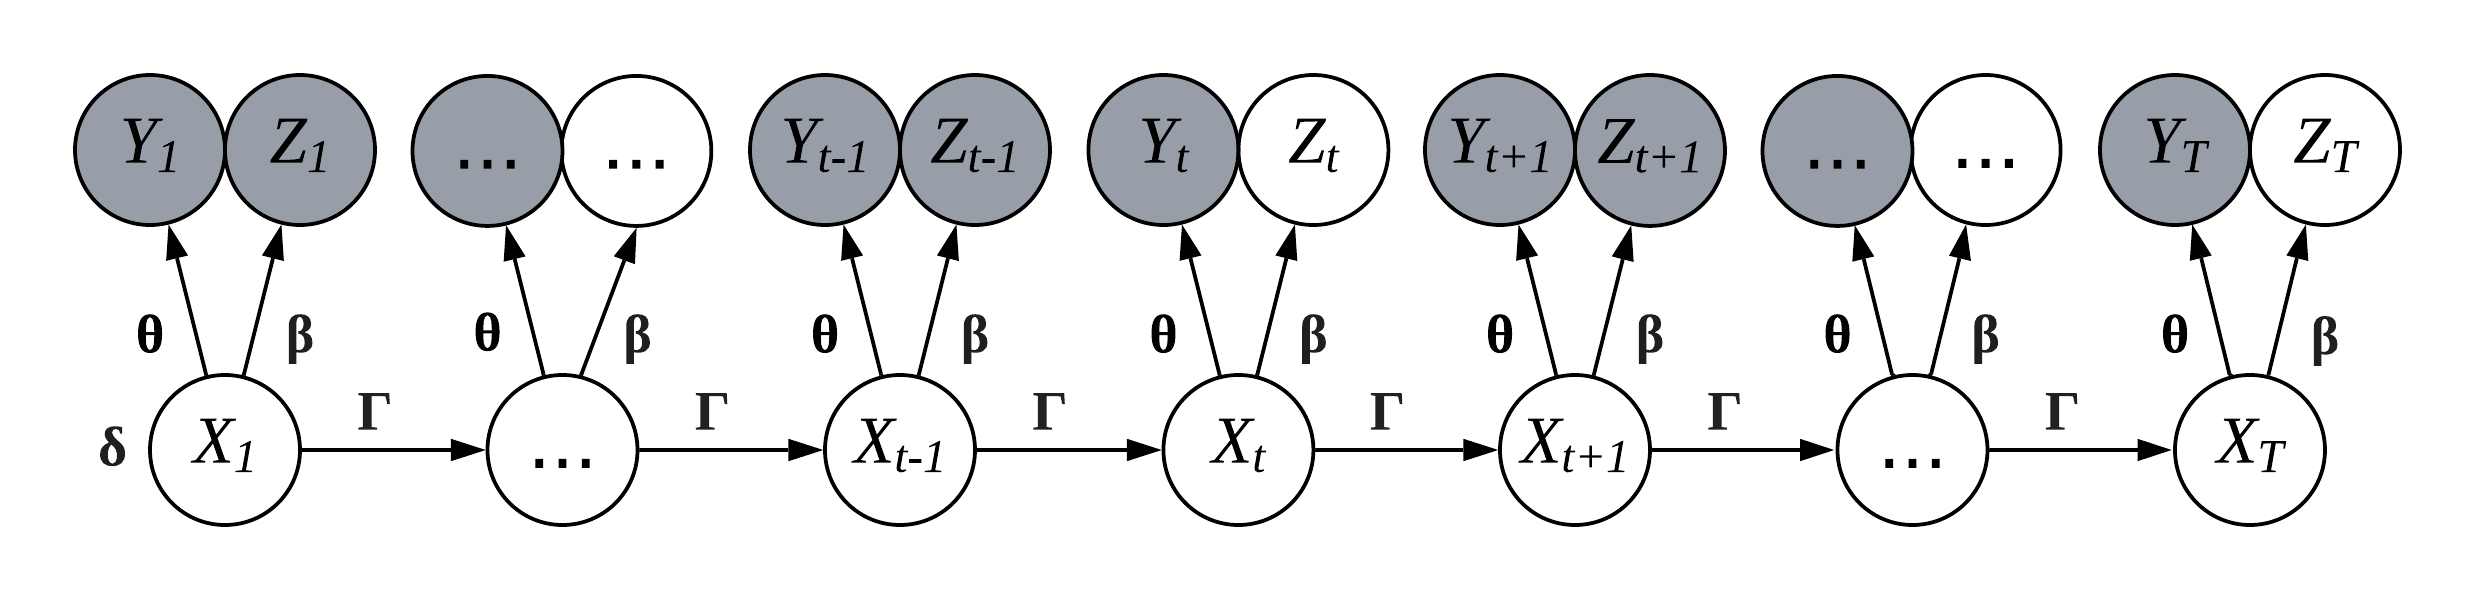
\includegraphics[width = 6in]{plt/PHMM_alpha_one.png}
        \caption{Partially hidden Markov model with $\alpha = 1$. This PHMM gives equal weight to all observations in the likelihood function. This is the ``natural" formulation of a PHMM with missing labels.}
    \end{subfigure}%
    \\
    \begin{subfigure}[t]{\textwidth}
        \centering
        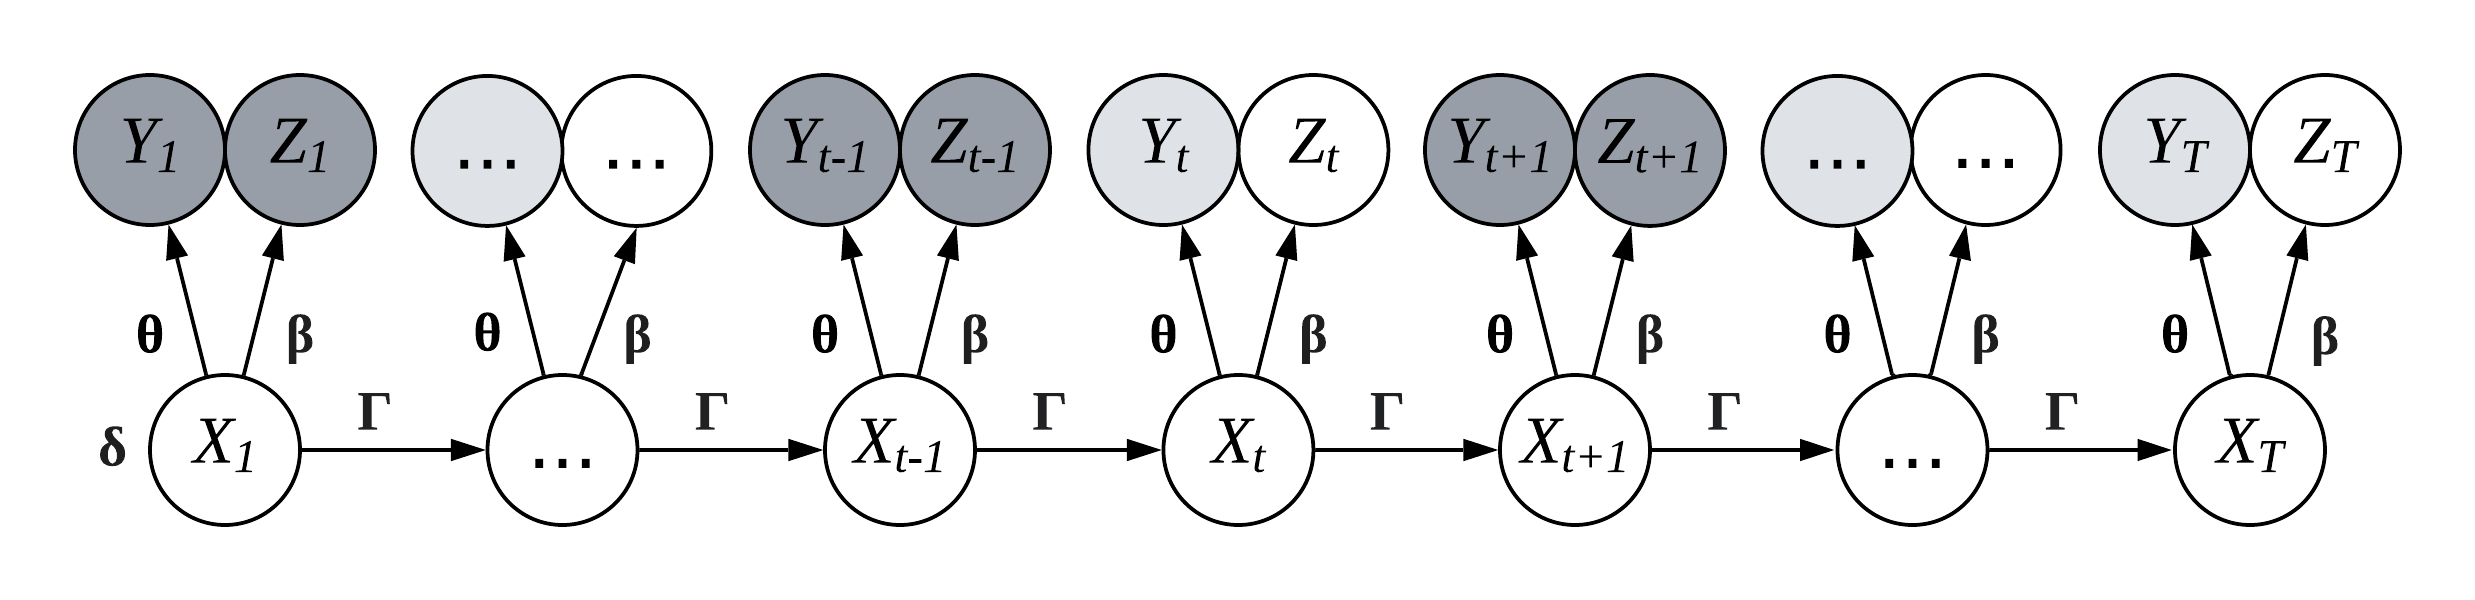
\includegraphics[width = 6in]{plt/PHMM_alpha_half.png}
        \caption{Partially hidden Markov model with $\alpha \in (0,1)$. This PHMM weights the influence of $Y_t$, $Y_T$, and all other observations that do not have associated observed labels. However, it does not ignore them altogether.}
    \end{subfigure}%
    \\
    \begin{subfigure}[t]{\textwidth}
        \centering
        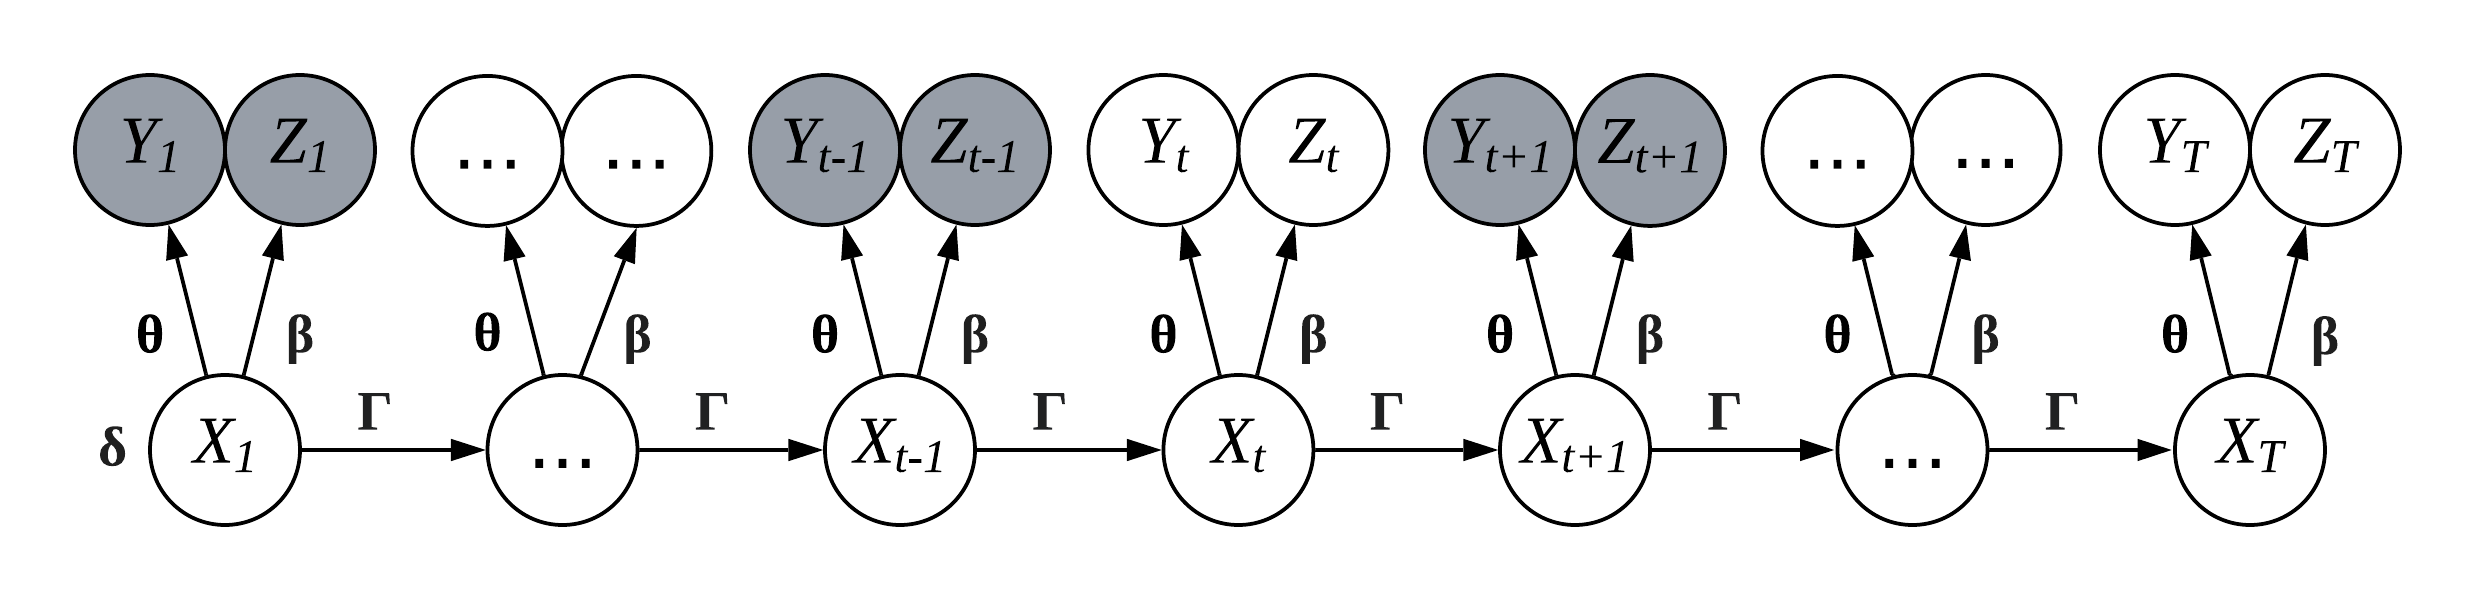
\includegraphics[width = 6in]{plt/PHMM_alpha_zero.png}
        \caption{Partially hidden Markov model with $\alpha = 0$. This PHMM ignores all observations that do not have associated label information. In particular, $Y_t$, $Y_T$, and all other observations that do not have observed labels are treated as unobserved.}
    \end{subfigure}%
    \caption{Graphical representation of various PHMMs with likelihood weightings (a) $\alpha = 1$, (b) $\alpha \in (0,1)$ and (c) $\alpha = 0$. The colour (white, light grey, and dark grey) indicates how much a given observation affects the weighted likelihood. White corresponds to treating the random variable as unobserved, dark grey corresponds to treating the variable as fully observed, and light grey corresponds to treating the random variable as observed, but weighting it in the likelihood. The latent states $\{X_{t'}\}_{t'=1}^{T}$, observations $\{Y_{t'}\}_{t'=1}^{T}$, and labels $\{Z_{t'}\}_{t'=1}^{T}$ are as described in Section \ref{sec:model}. %$X_t$ corresponds to an unobserved latent state at time $t$ whose distribution is described by a Markov chain. $Y_t$ corresponds to an observation at time $t$, where $Y_t$ given all other observations $\bfY \setminus \{Y_t\}$, hidden states $\bfX$, and labels $\bfZ$ depends only on $X_t$. Similarly, $Z_t$ corresponds to the label at time $t$, where $Z_t$ given all observations $\bfY$, hidden states $\bfX$, and other labels $\bfZ \setminus \{Z_t\}$ depends only on $X_t$. 
    In this example, $Z_1$, $Z_{t-1}$, and $Z_{t+1}$ are observed, while all other labels are unobserved (i.e., $Z_{t'} = \emptyset$ for $t' \neq 1,t-1,t+1$).}
    \label{fig:PHMM}
\end{figure}

I recommend that practitioners employ the following cross-validation procedure to find an optimal value of $\alpha$. First, select a range of candidate values of $\alpha \in [0,1]$. I in particular recommend testing at least $\alpha \in \{0,|\calT| / (T - |\calT|), 1\}$, as $\alpha = |\calT| / (T - |\calT|)$ approximately balances the influence of labelled and unlabelled observations in the likelihood. Second, divide the time series data set into several ``folds" for cross validation. Third, train the PHMM on the full data set while ignoring a fold, and use the forward-backward algorithm on the held-out fold (ignoring its associated labels) to estimate the hidden state probabilities $\bbP(X_t \mid \bfY = \bfy)$. Fourth, repeat the previous step for all folds to estimate the cross-validated hidden states probabilities for the entire data set. Finally, use the estimated probabilities and true labels together with standard model validation techniques to evaluate the resulting PHMM and select the most appropriate value of $\alpha$. %To solidify this idea and show the performance of the method, I used this process to conduct two case studies that are presented in the next section.
